\documentclass[tikz]{standalone}
    \usepackage{pgfplots}
    \pgfplotsset{compat=newest}

    \begin{document}

    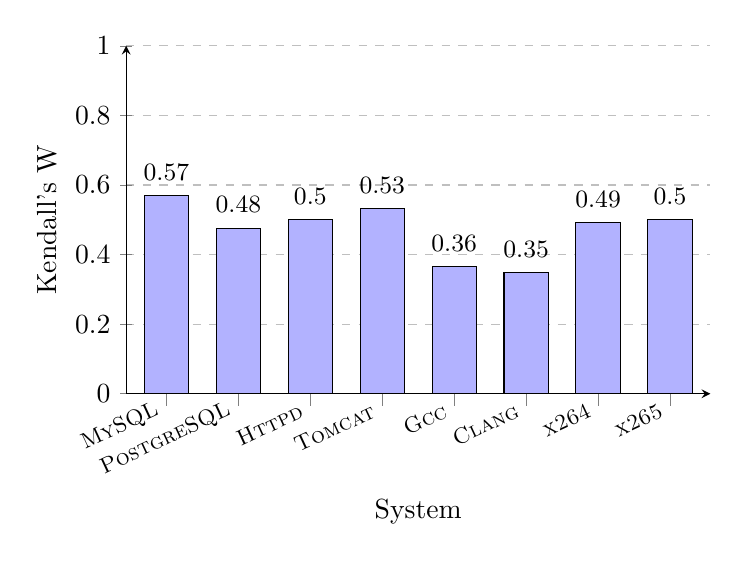
\begin{tikzpicture}
    \begin{axis}[
        height=6cm,
        width=9cm,
        grid style={dashed},
        ymajorgrids=true,
        axis x line=bottom,
        axis y line=left,
        ymin=0,
        ymax=1.0,
        enlarge x limits=0.08,
        ybar=0pt,
        bar width=16pt,
        ylabel={Kendall's W},
        xlabel={System},
        symbolic x coords={mysql,postgresql,httpd,tomcat,gcc,clang,x264,x265},
        xtick=data,
        xticklabels={\textsc{MySQL},\textsc{PostgreSQL},\textsc{Httpd},\textsc{Tomcat},\textsc{Gcc},\textsc{Clang},\textsc{x264},\textsc{x265}},
        xticklabel style={rotate=25, anchor=east, font=\footnotesize},
        y axis line style={black},
        yticklabel style={black},
        nodes near coords,
        every node near coord/.append style={font=\small, yshift=2pt},
        nodes near coords align={vertical},
    ]

\addplot[
    fill=blue!30,
    draw=black,
    opacity=1
]
coordinates {
(mysql,0.5701)
(postgresql,0.4755)
(httpd,0.5000)
(tomcat,0.5312)
(gcc,0.3648)
(clang,0.3474)
(x264,0.4914)
(x265,0.5003)
};

\end{axis}
\end{tikzpicture}

\end{document}
